\usetikzlibrary{arrows.meta}
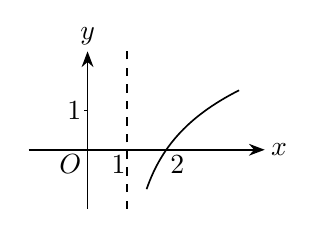
\begin{tikzpicture}[x=0.5cm,y=0.5cm,>=Stealth,line width=.6pt]
\coordinate (O) at (0,0);
\coordinate (Xleft) at (-1.5,0);
\coordinate (Xend) at (4.5,0);
\coordinate (Ylow) at (0,-1.5);
\coordinate (Yend) at (0,2.5);
\coordinate (P) at (2,0);
\coordinate (Q) at (1,0);
\draw[->] (Xleft)--(Xend);
\draw[->] (Ylow)--(Yend);
\draw[dashed] (1,-1.5)--(1,2.5);
\draw[domain=1.5:3.85,samples=120] plot (\x,{ln(\x-1)/ln(2)});
\draw (-0.08,1)--(0,1);
\node[below left,inner sep=0pt,xshift=-2pt,yshift=-1.5pt] at (O) {$O$};
\node[below,inner sep=0pt,yshift=-2pt,xshift=-3pt] at (1,0) {$1$};
\node[below,inner sep=0pt,yshift=-2pt,xshift=4pt] at (2,0) {$2$};
\node[left,inner sep=0pt,xshift=-2pt] at (0,1) {$1$};
\node[right,inner sep=0pt,xshift=2pt] at (Xend) {$x$};
\node[above,inner sep=0pt,yshift=2pt] at (Yend) {$y$};
\end{tikzpicture}
